% Propósito: distinguir el nivel medido en un punto de campo libre del nivel
% próximo al tímpano y mostrar que su diferencia es una transferencia
% dependiente de frecuencia, no una ganancia fija de sonoridad.
% Origen: G_CT(f)=L_p,T(f)-L_p,campo(f), ecuación
% \eqref{eq:u7-ganancia-campo-timpano}. Esquema geométrico sin escala.
% Descripción accesible: en el panel izquierdo una onda llega a un punto de
% referencia de campo libre sin oyente. En el panel derecho la misma onda llega
% a una cabeza esquemática; pabellón y canal conducen hacia el tímpano. Debajo
% se comparan los niveles en ambos puntos mediante la diferencia G_CT.
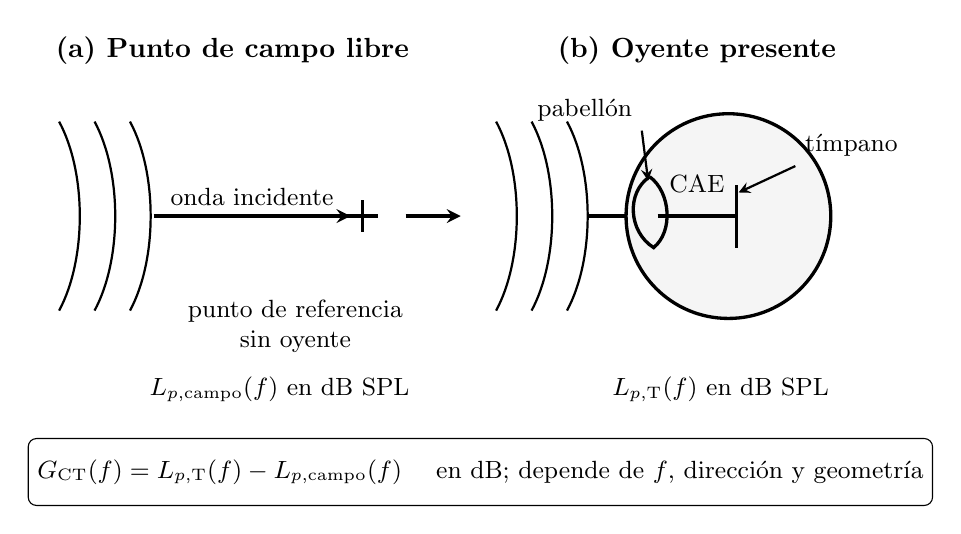
\begin{tikzpicture}[font=\small,>=stealth,x=1cm,y=1cm]
    \node[font=\bfseries] at (2.75,4.85)
        {(a) Punto de campo libre};
    \node[font=\bfseries] at (8.65,4.85)
        {(b) Oyente presente};

    % Panel (a).
    \foreach \xx in {0.55,1.00,1.45}{
        \draw[thick] (\xx,1.55) .. controls
            (\xx+0.35,2.20) and (\xx+0.35,3.30) .. (\xx,3.95);
    }
    \draw[->,very thick] (1.75,2.75) -- (4.25,2.75)
        node[midway,above] {onda incidente};
    \draw[very thick] (4.40,2.55) -- (4.40,2.95);
    \draw[very thick] (4.20,2.75) -- (4.60,2.75);
    \node[align=center] at (3.55,1.35)
        {punto de referencia\\sin oyente};
    \node[align=center] at (3.35,0.55)
        {\(L_{p,\mathrm{campo}}(f)\) en dB SPL};

    % Panel (b).
    \foreach \xx in {6.10,6.55,7.00}{
        \draw[thick] (\xx,1.55) .. controls
            (\xx+0.35,2.20) and (\xx+0.35,3.30) .. (\xx,3.95);
    }
    \draw[->,very thick] (7.25,2.75) -- (8.05,2.75);
    \draw[very thick,fill=black!4] (9.05,2.75) circle (1.30);
    \draw[very thick] (8.05,3.25)
        .. controls (7.75,3.05) and (7.78,2.55) .. (8.10,2.35)
        .. controls (8.35,2.55) and (8.32,3.05) .. (8.05,3.25);
    \draw[very thick] (8.15,2.75) -- (9.15,2.75);
    \draw[very thick] (9.15,2.35) -- (9.15,3.15);
    \node[anchor=east] (pinna-label) at (7.95,4.10) {pabellón};
    \draw[->,thick] (pinna-label.south east) -- (8.03,3.20);
    \node[anchor=south] at (8.65,2.92) {CAE};
    \node[anchor=west] (eardrum-label) at (9.90,3.65) {tímpano};
    \draw[->,thick] (eardrum-label.south west) -- (9.18,3.05);
    \node[align=center] at (8.95,0.55)
        {\(L_{p,\mathrm{T}}(f)\) en dB SPL};

    \draw[very thick,->] (4.95,2.75) -- (5.65,2.75);
    \node[align=center,draw,rounded corners=3pt,fill=white,
        minimum width=7.60cm,minimum height=0.85cm] at (5.90,-0.50)
        {\(\displaystyle
          G_{\mathrm{CT}}(f)
          =L_{p,\mathrm{T}}(f)-L_{p,\mathrm{campo}}(f)\)
         \quad en dB; depende de \(f\), dirección y geometría};
\end{tikzpicture}
